% remsi
\begin{figure}[H]
    \centering


\tikzset{every picture/.style={line width=0.75pt}} %set default line width to 0.75pt        

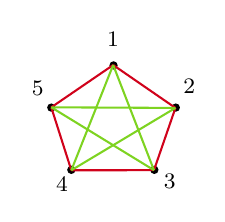
\begin{tikzpicture}[x=0.75pt,y=0.75pt,yscale=-1,xscale=1]
%uncomment if require: \path (0,300); %set diagram left start at 0, and has height of 300

%Shape: Free Drawing [id:dp7845526837677299] 
\draw  [line width=3] [line join = round][line cap = round] (170.13,120.13) .. controls (170.13,120.13) and (170.13,120.13) .. (170.13,120.13) ;
%Shape: Free Drawing [id:dp651820155137359] 
\draw  [line width=3] [line join = round][line cap = round] (210.13,120.13) .. controls (210.13,120.13) and (210.13,120.13) .. (210.13,120.13) ;
%Shape: Free Drawing [id:dp882216976010495] 
\draw  [line width=3] [line join = round][line cap = round] (220.47,90.13) .. controls (220.47,90.13) and (220.47,90.13) .. (220.47,90.13) ;
%Shape: Free Drawing [id:dp6878741057741864] 
\draw  [line width=3] [line join = round][line cap = round] (160.47,90.13) .. controls (160.47,90.13) and (160.47,90.13) .. (160.47,90.13) ;
%Shape: Free Drawing [id:dp35491147937374956] 
\draw  [line width=3] [line join = round][line cap = round] (190.47,69.8) .. controls (190.47,69.8) and (190.47,69.8) .. (190.47,69.8) ;
%Straight Lines [id:da036432670890108154] 
\draw [color={rgb, 255:red, 208; green, 2; blue, 27 }  ,draw opacity=1 ]   (160.47,90) -- (170.13,120.33) ;
%Straight Lines [id:da8177956817637941] 
\draw [color={rgb, 255:red, 208; green, 2; blue, 27 }  ,draw opacity=1 ]   (190.29,69.62) -- (160.47,90) ;
%Straight Lines [id:da3135487515788027] 
\draw [color={rgb, 255:red, 208; green, 2; blue, 27 }  ,draw opacity=1 ]   (170.13,120.33) -- (209.95,120.29) ;
%Straight Lines [id:da4204459432952701] 
\draw [color={rgb, 255:red, 208; green, 2; blue, 27 }  ,draw opacity=1 ]   (190.29,69.62) -- (220.29,90.29) ;
%Straight Lines [id:da006642295475887572] 
\draw [color={rgb, 255:red, 208; green, 2; blue, 27 }  ,draw opacity=1 ]   (220.29,90.29) -- (209.95,120.29) ;
%Straight Lines [id:da28150454662534186] 
\draw [color={rgb, 255:red, 126; green, 211; blue, 33 }  ,draw opacity=1 ]   (190.29,69.62) -- (209.95,120.29) ;
%Straight Lines [id:da012896293421401639] 
\draw [color={rgb, 255:red, 126; green, 211; blue, 33 }  ,draw opacity=1 ]   (160.47,90) -- (209.95,120.29) ;
%Straight Lines [id:da4519195166670298] 
\draw [color={rgb, 255:red, 126; green, 211; blue, 33 }  ,draw opacity=1 ]   (170.13,120.33) -- (190.29,69.62) ;
%Straight Lines [id:da9239288264644911] 
\draw [color={rgb, 255:red, 126; green, 211; blue, 33 }  ,draw opacity=1 ]   (160.47,90) -- (220.29,90.29) ;
%Straight Lines [id:da7006912451897753] 
\draw [color={rgb, 255:red, 126; green, 211; blue, 33 }  ,draw opacity=1 ]   (170.13,120.33) -- (220.29,90.29) ;

% Text Node
\draw (185.93,52.13) node [anchor=north west][inner sep=0.75pt]  [font=\footnotesize] [align=left] {1};
% Text Node
\draw (222.6,75.13) node [anchor=north west][inner sep=0.75pt]  [font=\footnotesize] [align=left] {2};
% Text Node
\draw (213.27,120.8) node [anchor=north west][inner sep=0.75pt]  [font=\footnotesize] [align=left] {3};
% Text Node
\draw (161.27,122.13) node [anchor=north west][inner sep=0.75pt]  [font=\footnotesize] [align=left] {4};
% Text Node
\draw (149.6,75.8) node [anchor=north west][inner sep=0.75pt]  [font=\footnotesize] [align=left] {5};


\end{tikzpicture}
    
\end{figure}